% ===========================================================================
% CAPÍTULO 3 — DESARROLLO: las tres arquitecturas de transporte PS<->PL
% ===========================================================================

\section{Arquitecturas de transporte PS--PL} \label{sec:transporte_desarrollo}

El factor que determina el rendimiento del sistema con los catorce canales activos no es el
transceptor ni el software del driver, sino \textbf{el camino por el que los bytes viajan entre la
DDR y la lógica programable}: en la arquitectura de partida cada byte recibido genera una
interrupción, y el procesador no da abasto con las catorce líneas.

Para determinar con datos cuál es la arquitectura de transporte PS--PL adecuada para catorce
líneas serie sobre este MPSoC se implementaron \textbf{tres arquitecturas completas}, resumidas
en la tabla~\ref{tab:tres_variantes}, y se midieron con el mismo programa de pruebas. El
transceptor serie de la sección anterior es idéntico en las tres; lo único que cambia es el
transporte y el driver \texttt{transceiver.c/h} que lo maneja.

\begin{table}[H]
    \centering
    \begin{tabular}{p{2.9cm} p{5.0cm} p{6.1cm}}
        \hline
        \textbf{Variante} & \textbf{Transporte PS$\leftrightarrow$PL} & \textbf{Idea} \\
        \hline
        A --- GPIO & AXI-Lite / AXI GPIO & Un registro por canal; el PS mueve byte a byte. \\
        B --- DMA14 & 14 $\times$ AXI DMA (PG021) & Un motor DMA completo por canal. \\
        C --- MCDMA & 1 $\times$ AXI MCDMA (PG288) + puente VHDL & Un motor multicanal compartido. \\
        \hline
    \end{tabular}
    \caption{Las tres arquitecturas de transporte implementadas y comparadas.}
    \label{tab:tres_variantes}
\end{table}

Las tres son funcionales y arrancan sobre la misma placa con el mismo código de aplicación.
El capítulo de resultados (sección~\ref{sec:resultados_benchmark}) recoge la comparativa
cuantitativa; esta sección describe la construcción de cada una.

% ---------------------------------------------------------------------------
\subsection{Variante A --- AXI GPIO (referencia)}
% ---------------------------------------------------------------------------

Es la arquitectura de partida, la descrita en las secciones anteriores de este capítulo, y la
referencia contra la que se mide todo lo demás. Cada canal es una instancia de
\texttt{CONFIGURABLE\_SERIAL\_TOP} con su propio AXI GPIO de doble canal, colgado de un
\textit{smartconnect} AXI-Lite: un registro de escritura (dato de transmisión, bits de control y
configuración de protocolo) y un registro de lectura (dato recibido y banderas de estado). Un AXI
INTC concentra las veintiocho fuentes de interrupción (RX y TX de cada canal) en una sola línea
hacia el PS.

Su virtud es la simplicidad: es la variante con menos lógica, no necesita ningún mapeo especial
de la MMU y no tiene que preocuparse por la coherencia de caché, porque todos los accesos son
del propio procesador. Su defecto es estructural y no tiene arreglo dentro de esta
arquitectura: \textbf{el procesador tiene que tocar cada byte}. En recepción, cada carácter
completo genera una interrupción; la ISR maestra despierta a la tarea \textit{worker} del canal,
que drena el FIFO hardware byte a byte. En transmisión, la ISR escribe el siguiente byte cada
vez que el transmisor queda libre.

El coste medido es de \textbf{1\,250 interrupciones por kilobyte} transferido. Con eso, el
\textit{throughput} de un canal se estanca en torno al 30\,\% del techo físico de la línea y
\textbf{no mejora al subir la velocidad}: de 115\,200 a 4~Mbaudios
el rendimiento apenas pasa de 3\,471 a 4\,907~B/s, porque el cuello de botella ya no es la línea
serie sino el manejo de interrupciones. El sistema está en el régimen de \textit{interrupt
livelock} descrito en la sección~\ref{sec:teoria_livelock}.

% ---------------------------------------------------------------------------
\subsection{Variante B --- 14$\times$ AXI DMA}
% ---------------------------------------------------------------------------

Esta variante saca a la CPU del movimiento de datos delegándolo en motores DMA. Como un
\texttt{axi\_dma} sirve a un único \textit{stream}, cubrir los catorce canales exige catorce
instancias.

\subsubsection{Adaptación del UART a AXI-Stream}

El transceptor original habla con registros, no con \textit{streams}. El módulo
\texttt{UART\_AXIS\_TOP.vhd} hace de adaptador: envuelve un \texttt{CONFIGURABLE\_SERIAL} y le
añade una interfaz AXI4-Stream esclava en el lado de transmisión (\texttt{TDATA},
\texttt{TVALID}, \texttt{TREADY}) y una maestra en el de recepción (con \texttt{TLAST} para
delimitar el paquete). Cada uno de los catorce UART se convierte así en un periférico
AXI-Stream que cuelga de su propio DMA.

\subsubsection{Operación}

Los DMA se configuran en modo directo, sin \textit{scatter-gather}, que es todo lo que necesita
un canal con un único \textit{buffer} activo:

\begin{itemize}
    \item \textbf{Transmisión.} El driver escribe la dirección del \textit{buffer} y la longitud
    en los registros del canal MM2S; el motor lee la DDR y alimenta el \textit{stream}. La ISR
    de MM2S libera un semáforo al completar la transferencia.
    \item \textbf{Recepción.} El canal S2MM se arma con longitud 1. El \texttt{TLAST} que el
    adaptador emite con cada byte completa el paquete, la ISR de S2MM copia el dato al
    \textit{ring} de software y rearma el descriptor.
\end{itemize}

\subsubsection{Coste de la replicación de motores DMA}

La variante opera en placa y en transmisión alcanza \textbf{3 interrupciones por kilobyte}, frente
a las 1\,250 de la variante GPIO. El límite de la variante no está, por tanto, en el rendimiento
que alcanza, sino en el precio que paga por alcanzarlo. Replicar catorce veces el motor DMA choca
con dos recursos finitos del dispositivo:

\textbf{El coste en lógica.} Catorce motores DMA completos ocupan \textbf{40\,217 LUT}
(\textit{Look-Up Table}), un 14,7\,\% del dispositivo: 2,8 veces más lógica que la solución
multicanal, para el mismo número de canales. La cifra por canal, 2\,873 LUT/canal frente a los 1\,014 del MCDMA, expresa
directamente lo que cuesta replicar en vez de compartir. Ese coste condiciona además
el endurecimiento futuro del diseño, porque una triplicación modular (TMR, \textit{Triple Modular
Redundancy}) de la lógica, que es la técnica habitual para tolerar los efectos de la radiación en
órbita, multiplicaría por tres esa huella y la llevaría a cerca de la mitad del dispositivo,
mientras que sobre la variante multicanal sigue siendo asumible.

\textbf{El límite de las interrupciones.} Cada \texttt{axi\_dma} expone dos líneas de
interrupción, MM2S y S2MM. Catorce DMA son \textbf{veintiocho líneas}, y el PS solo ofrece ocho
en \texttt{pl\_ps\_irq0}. Hubo que reducirlas por OR en la propia PL hasta dejarlas en dos, con
lo que la ISR pierde la información de \textit{qué} canal ha interrumpido y debe escanear los
catorce registros de estado en cada evento. El ahorro de interrupciones que aportaba el DMA se
paga en parte con un coste de escaneo dentro de la ISR.

El límite de ocho líneas es del dispositivo, no del diseño, y no se resuelve replicando más
motores: es la restricción que conduce a la tercera variante.

La recepción de esta variante \textbf{no llegó a medirse}. El banco de pruebas de la
sección~\ref{sec:bench_loopback} exige insertar el módulo de \textit{loopback} en el diseño de
cada variante, y sobre esta el lazo de recepción no llegó a operar: el autodiagnóstico del banco
lo señaló como abierto y todos los tests que dependen de recibir salieron a cero. Con el coste en
lógica y el límite de líneas de interrupción ya medidos, la arquitectura quedaba descartada como
solución final con independencia de lo que midiera su recepción, por lo que la depuración no se
llevó más allá y el esfuerzo se dedicó al diseño de la variante MCDMA. Sus cifras de recepción
constan como no disponibles en los resultados; las válidas de esa corrida son el coste de
hardware, la huella de memoria y las interrupciones de transmisión.

% ---------------------------------------------------------------------------
\subsection{Variante C --- AXI MCDMA con puente VHDL}
% ---------------------------------------------------------------------------

La tercera arquitectura, y la que se adopta como solución final, sustituye los catorce motores
por \textbf{uno solo multicanal} (\texttt{axi\_mcdma}, PG288) y añade un \textbf{puente en VHDL}
que reparte y recoge de los catorce UART. Es la variante con más diseño propio y la única en la
que el problema deja de resolverse instanciando IP de terceros.

La topología es deliberadamente \textbf{asimétrica}, porque los dos sentidos tienen exigencias
distintas:

\begin{itemize}
    \item En \textbf{transmisión} el PS decide cuándo y a quién escribe. Basta con un canal DMA
    si el destino viaja \textit{dentro} del dato.
    \item En \textbf{recepción} los catorce canales pueden hablar a la vez y sin avisar. Cada uno
    necesita su propio \textit{buffer} en la DDR para que los flujos no se mezclen, lo que exige
    catorce canales S2MM.
\end{itemize}

De ahí la asimetría de la figura~\ref{fig:mcdma_bd}: un solo canal en el sentido de transmisión y
catorce en el de recepción, sobre un mismo motor multicanal.

\begin{sidewaysfigure}
    \centering
    \figpendiente{IMG/Desarrollo/diagrama_arquitectura_mcdma.pdf}{0.97\textheight}{arquitectura
    completa de la solución final --- DDR y RTEMS en el PS; \texttt{axi\_mcdma} con 1 canal MM2S
    y 14 canales S2MM; conversores de anchura 32$\rightarrow$8 y 8$\rightarrow$32;
    \texttt{BRIDGE\_TX\_TOP} y \texttt{BRIDGE\_RX\_TOP}; los 14 transceptores serie;
    \texttt{TX\_ISR\_EOF\_HANDLER} y las tres líneas de interrupción; y las líneas
    TD/RD/DE/SLO hacia la PCB}
    \caption{Arquitectura de la variante MCDMA.}
    \label{fig:mcdma_bd}
\end{sidewaysfigure}

\subsubsection{Camino de transmisión}

El canal MM2S del MCDMA emite un único \textit{stream} de 32 bits, que un conversor de anchura
reduce a 8. Con un solo canal de DMA, \textbf{el destino de cada byte viaja en la cabecera del
propio paquete}:

\begin{center}
\texttt{[ \{CH\_ID[3:0], LEN[11:8]\} | \{LEN[7:0]\} | payload\ldots ]}
\end{center}

Dos bytes de cabecera con el identificador de canal y la longitud del \textit{payload}. El
bloque \texttt{BRIDGE\_TX\_TOP} los interpreta y encamina el resto del paquete:

\begin{itemize}
    \item \texttt{TX\_DMA\_ROUTER} parsea la cabecera y extrae el canal y la longitud.
    \item \texttt{MUX\_2x16} demultiplexa la escritura hacia la FIFO del canal indicado.
    \item Catorce \texttt{TX\_WORKER}, uno por canal, con una FIFO de 8 bits en modo
    \textit{first-word-fall-through} y una máquina de estados (\texttt{S\_IDLE} $\rightarrow$
    \texttt{S\_START} $\rightarrow$ \texttt{S\_BUSY}) que alimenta el núcleo UART byte a byte,
    respetando su \textit{handshake}: presenta el byte, espera a que el transmisor lo acepte
    (\texttt{Send\_ok}), lo extrae de la FIFO y espera a que termine de serializarlo
    (\texttt{TX\_RDY}) antes de presentar el siguiente.
\end{itemize}

Un único canal DMA sirve así a los catorce transceptores. El precio es que las transmisiones se
serializan: el driver protege el acceso al canal compartido con un \textit{mutex}, y por eso
esta variante es la única en la que \texttt{Transceiver\_Send} es bloqueante.

\subsubsection{Notificación de fin de transmisión (\texttt{TX\_ISR\_EOF\_HANDLER})}

El DMA sabe cuándo ha terminado de \textit{entregar} el paquete al puente, pero no cuándo el
UART ha terminado de \textit{emitirlo} por el cobre. Para una línea RS-485 con control de
dirección esa diferencia importa: no se puede soltar el bus antes de que el último bit haya
salido.

Sacar los catorce pulsos de fin de trama a catorce líneas de interrupción no es una opción
porque las líneas son ocho. Se diseñó por tanto un bloque propio,
\texttt{TX\_ISR\_EOF\_HANDLER.vhd}, que aplica el patrón de \textbf{registro \textit{sticky} más
una única interrupción}: engancha el pulso de fin de trama de cada \textit{worker} en un bit de
un registro, lo expone por AXI-Lite y genera una sola interrupción de nivel. Su mapa de
registros es el de la tabla~\ref{tab:tx_isr_regs}:

\begin{table}[H]
    \centering
    \begin{tabular}{llll}
        \hline
        \textbf{Offset} & \textbf{Registro} & \textbf{Acceso} & \textbf{Función} \\
        \hline
        \texttt{0x00} & \texttt{TX\_DONE}       & RO  & Un bit por canal; se pone a 1 al fin de trama. \\
        \texttt{0x04} & \texttt{TX\_DONE\_CLEAR} & W1C & Escribir 1 borra el bit correspondiente. \\
        \texttt{0x08} & \texttt{IRQ\_ENABLE}    & RW  & Máscara de canales que generan interrupción. \\
        \texttt{0x0C} & \texttt{IRQ\_STATUS}    & RO  & \texttt{TX\_DONE} \texttt{AND} \texttt{IRQ\_ENABLE}. \\
        \hline
    \end{tabular}
    \caption{Mapa de registros del bloque \texttt{TX\_ISR\_EOF\_HANDLER} (base \texttt{0xA0001000}).}
    \label{tab:tx_isr_regs}
\end{table}

La interrupción es el OR de los bits habilitados, y la puesta a 1 por fin de trama tiene
prioridad sobre el borrado por software, para que no se pierda un evento que llegue justo
durante la escritura de \textit{clear}. El driver espera en un semáforo que esta ISR libera, de
modo que \texttt{Transceiver\_Send} retorna cuando el byte ha salido físicamente, no cuando el
DMA lo ha copiado.

\subsubsection{Camino de recepción y etiquetado por TDEST}

En recepción cada UART entrega bytes de forma autónoma. El bloque \texttt{BRIDGE\_RX\_TOP}
recoge los catorce flujos y los presenta al MCDMA como un único \textit{stream} etiquetado:

\begin{itemize}
    \item Una \textbf{FIFO por canal} absorbe la ráfaga de bytes que llega mientras el árbitro
    atiende a otro.
    \item Un \textbf{DEMUX} recorre las catorce FIFO.
    \item El bloque \textbf{DRAIN} vacía la FIFO seleccionada hacia el \textit{stream} de salida,
    cierra el paquete con \texttt{TLAST} y fija el \textbf{\texttt{TDEST}} con el número de canal de
    procedencia.
\end{itemize}

El MCDMA demultiplexa por \texttt{TDEST}: el paquete etiquetado con el canal $N$ acaba en el
descriptor y el \textit{buffer} de DDR del canal $N$. Sin esa etiqueta el hardware no tiene forma
de saber de quién es cada byte, y todo el tráfico se deposita en el canal cero, comportamiento
que se documenta en la sección~\ref{sec:transporte_depuracion}.

La figura~\ref{fig:mcdma_interior} recoge el mecanismo completo. Los catorce canales entran y
salen por un único par de interfaces AXI-Stream, y es la etiqueta \texttt{TDEST} la que decide en
qué \textit{buffer} de la DDR acaba cada paquete.

\begin{figure}[htbp]
    \centering
    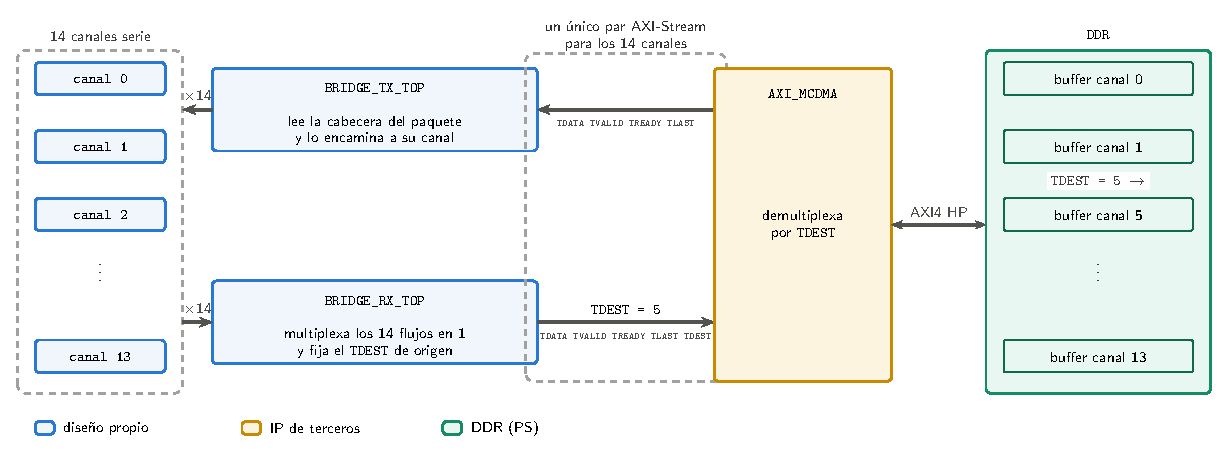
\includegraphics[width=\textwidth]{IMG/Desarrollo/diagrama_mcdma_interior.pdf}
    \caption{Multiplexado de los catorce canales por \texttt{TDEST}.}
    \label{fig:mcdma_interior}
\end{figure}

El paquete se cierra por dos condiciones: cuando la FIFO del canal se vacía (fin natural de la
ráfaga) o cuando se alcanza el tope duro de longitud del generic \texttt{MAX\_PKT}, fijado en
256~bytes. Ese segundo criterio es una \textbf{invariante de seguridad} impuesta por el IP, cuya
razón se detalla más abajo.

\subsubsection{Mapa de memoria y de interrupciones}

Los tres bloques que el PS debe alcanzar se sitúan en el mapa de memoria como recoge la
tabla~\ref{tab:mcdma_map}.

\begin{table}[H]
    \centering
    \begin{tabular}{lll}
        \hline
        \textbf{Dirección} & \textbf{Bloque} & \textbf{Tamaño} \\
        \hline
        \texttt{0xA000\_0000} & \texttt{AXI\_UART\_CONFIG} --- un registro de 32 bits por canal & 4~KB \\
        \texttt{0xA000\_1000} & \texttt{TX\_ISR\_EOF\_HANDLER} & 4~KB \\
        \texttt{0xA001\_0000} & Registros de control del \texttt{axi\_mcdma} & 64~KB \\
        \hline
    \end{tabular}
    \caption{Mapa de memoria de la variante MCDMA.}
    \label{tab:mcdma_map}
\end{table}

Las tres líneas de interrupción hacia el PS son \texttt{mm2s\_introut} (SPI 89, vector 121 en
RTEMS), \texttt{s2mm\_introut} (SPI 90, vector 122) y la del bloque propio de fin de trama (SPI
91, vector 123). Las catorce salidas de interrupción de los canales S2MM se reducen por OR a una
sola línea, y la ISR escanea los registros de estado para saber qué canales han completado.

\subsubsection{Construcción de descriptores \textit{scatter-gather} en el driver}

El MCDMA opera siempre en modo \textit{scatter-gather}, de modo que el driver de esta variante
no escribe direcciones en registros, sino que \textbf{construye descriptores en memoria}. Cada
BD ocupa 64~bytes alineados a 64, con la estructura de la tabla~\ref{tab:mcdma_bd}, y el driver
mantiene un anillo de un solo descriptor por canal, cuyo puntero al siguiente apunta a sí mismo:

\begin{table}[H]
    \centering
    \begin{tabular}{lll}
        \hline
        \textbf{Offset} & \textbf{Campo} & \textbf{Contenido} \\
        \hline
        \texttt{+0x00} & \texttt{NDESC}   & Dirección del siguiente descriptor (aquí, él mismo). \\
        \texttt{+0x08} & \texttt{BUFA}    & Dirección del \textit{buffer} de datos. \\
        \texttt{+0x14} & \texttt{CTRL}    & \texttt{SOF} (bit 31), \texttt{EOF} (bit 30), longitud (bits 25:0). \\
        \texttt{+0x18} & \texttt{STS}     & Recepción: \texttt{COMPLETE} (bit 31) y bytes realmente escritos. \\
        \texttt{+0x1C} & \texttt{SIDEBAND} & Transmisión: \texttt{COMPLETE} (bit 31). \\
        \hline
    \end{tabular}
    \caption{Estructura del descriptor de buffer (BD) del MCDMA.}
    \label{tab:mcdma_bd}
\end{table}

Rearmar un canal de recepción consiste en borrar el campo de estado, volcar la línea de caché
del descriptor y volver a escribir el puntero de cola: el motor lo relee y reanuda. La
recepción entrega el paquete cuando el puente cierra el \texttt{TLAST}, no byte a byte, que es
justamente el origen de la reducción de interrupciones.

% ---------------------------------------------------------------------------
\subsection{Verificación y depuración iterativa del driver} \label{sec:transporte_depuracion}
% ---------------------------------------------------------------------------

El driver descrito en las páginas anteriores es el resultado de \textbf{varias iteraciones} de una
metodología de verificación aplicada de forma sistemática a lo largo del trabajo:

\begin{enumerate}
    \item \textbf{Verificación aislada en simulación.} Ningún bloque de la PL se integraba en el
    diseño sin pasar antes su propio \textit{testbench} en Vivado. El puente y el módulo de
    \textit{loopback} tienen bancos de prueba dedicados que ejercitan el protocolo AXI-Stream y
    la topología de buses, respectivamente.
    \item \textbf{Integración incremental.} Cada bloque validado se incorporaba al diseño de
    bloques y se comprobaba de nuevo en placa antes de añadir el siguiente, para que cualquier
    regresión quedara acotada a la última pieza introducida.
    \item \textbf{Batería de pruebas automáticas en placa.} La aplicación de \textit{benchmark}
    (sección~\ref{sec:bench_loopback}) actúa como prueba de regresión del sistema completo: una
    campaña de treinta y seis comprobaciones cuyo resultado, cuántas pasan y cuáles fallan,
    dirigía la siguiente iteración.
\end{enumerate}

Las primeras iteraciones del driver resolvieron cuestiones de integración relativamente directas:
una versión inicial por \textit{polling}, que se sustituyó por un modelo íntegramente dirigido por
interrupción una vez el IP se regeneró con la interrupción por canal habilitada
(\texttt{c\_enable\_multi\_intr}); y la propagación de la señal \texttt{TDEST} a lo largo de toda
la jerarquía VHDL, sin la cual el MCDMA no puede demultiplexar y todo el tráfico de recepción
acaba atribuido al canal cero.

La parte más costosa fue la \textbf{depuración del bus AXI-Stream contra el motor de la DMA}. Los fallos de este bus no se manifiestan como un error:
no hay bit de estado, ni interrupción, ni descriptor marcado; el motor simplemente deja de
aceptar datos y el canal enmudece a mitad de una transferencia. Esa ausencia total de
observabilidad desde el software hace que depurar sobre la placa sea inviable, y obligó a
\textbf{reproducir el escenario en simulación}. Fueron necesarias numerosas iteraciones de
\textit{testbench}, inyectando contrapresión, paquetes de distinto tamaño y ráfagas
solapadas, hasta poder observar el \textit{handshake} congelándose ciclo a ciclo e identificar
las dos condiciones que lo provocaban.

De esas simulaciones salieron las dos \textbf{invariantes estructurales} que la lógica del puente
garantiza hoy por construcción:

\begin{itemize}
    \item \textbf{Tamaño de paquete acotado.} El motor de recepción está configurado en modo
    \textit{store-and-forward} (\texttt{c\_include\_s2mm\_sf~=~1}), de modo que acumula el paquete
    AXI-Stream completo en un \textit{buffer} interno de \textbf{512~bytes} antes de volcarlo a la
    DDR; un paquete mayor que ese \textit{buffer} lo bloquea indefinidamente, a la espera de un
    \texttt{TLAST} que ya no puede llegar. El bloque \texttt{DRAIN} impone por ello un tope duro
    \texttt{MAX\_PKT~=~256}, la mitad del \textit{buffer}, además de cerrar el paquete cuando la
    FIFO se vacía. El tope por longitud no es redundante: hace que la invariante sea estructural y
    no dependa de que el drenado gane siempre la carrera a la línea serie.
    \item \textbf{\texttt{TLAST} registrado.} La señal de fin de paquete no puede ser
    combinacional sobre el estado de «FIFO vacía» mientras hay un dato ofrecido. Si un byte nuevo
    llegara durante una espera por contrapresión, tumbaría el \texttt{TLAST} ya presentado,
    reabriendo el paquete y devolviendo el sistema al mismo bloqueo. La señal se congela en cuanto
    el byte se ofrece.
\end{itemize}

Con ambas incorporadas, el \textit{testbench} del puente de recepción,
\texttt{tb\_bridge\_rx.vhd}, pasa la batería completa. Sus cuatro pruebas están escogidas para
cubrir justamente los casos que provocaban el bloqueo: un canal aislado, tres canales
entremezclados, un paquete de 256~bytes que fuerza el cierre por longitud y dos ráfagas seguidas
sobre el mismo canal. Un \textit{scoreboard} comprueba byte a byte el \texttt{TDEST} de la
cabecera, que el canal esté en rango y que el dato coincida con el inyectado:

\begin{lstlisting}[basicstyle=\ttfamily\scriptsize, caption={Salida de la simulación de \texttt{tb\_bridge\_rx.vhd}}]
-- Reset liberado --
T1: canal unico ch2 (3 bytes, timeout)
T2: multi-canal ch0/ch5/ch13 (1 byte c/u, timeout)
T3: 256 bytes ch1, prog_full auto-trigger
T4: back-to-back ch7 (2 eventos de timeout)
------------------------------------------------------------
Checks totales  : 802
Errores         : 0
Pendientes exp  : 0
------------------------------------------------------------
SIM_RESULT: PASS
\end{lstlisting}

El contador de \textit{pendientes} a cero es tan relevante como el de errores: significa que no
quedó ni un byte inyectado sin salir por el \textit{stream}, que es el síntoma del bloqueo
descrito.

Por encima de esa prueba de bloque, \texttt{tb\_system\_e2e.vhd} cierra el lazo completo en
simulación (MCDMA $\rightarrow$ puente de transmisión $\rightarrow$ transceptor serie
$\rightarrow$ realimentación de la línea $\rightarrow$ puente de recepción $\rightarrow$ MCDMA),
configurando los canales a 921\,600~8N1 y comprobando que cada byte reaparece etiquetado con su
canal de origen:

\begin{lstlisting}[basicstyle=\ttfamily\scriptsize, caption={Salida de la simulación del sistema completo, \texttt{tb\_system\_e2e.vhd}}]
[CONFIG] Escribiendo 921600 8N1 en canales 0 y 1...
[TEST-1] TX->CH0 loopback: 0xA5, 0x3C ...
[TEST-1] PASS
[TEST-2] TX->CH0(0xDE) y CH1(0xAD) simultaneo...
[TEST-2] PASS
[TEST-3] Inyeccion serie directa CH1 <- 0x55 ...
[TEST-3] PASS
SIM_RESULT: PASS
\end{lstlisting}

El TEST-2 verifica el demultiplexado por \texttt{TDEST} con dos canales hablando a la vez, que es
la condición que en placa se manifestaba como «todo el tráfico acaba en el canal cero».

El flujo de trabajo impone además una comprobación adicional. El bloque que engloba el puente y
los transceptores está integrado como \textit{module reference}, y Vivado \textbf{cachea su
\textit{checkpoint}} de síntesis fuera de contexto. Editar el VHDL y relanzar la implementación
no cambia el \textit{bitstream}: el flujo termina sin aviso, cierra \textit{timing} y escribe un
\texttt{.bit} con el RTL antiguo. La comprobación quedó incorporada al procedimiento: verificar
que el \textit{hash} del \texttt{BOOT.bin} cambia antes de dar por bueno un \textit{bitstream}
nuevo.

Con estas correcciones el driver quedó estable: la campaña completa pasó de \textbf{0 de 36} a
\textbf{36 de 36} comprobaciones, la prueba de \textit{throughput} entrega los 5120 bytes de las
cinco repeticiones sin pérdidas y el barrido de velocidad supera los siete puntos, de 115\,200 a
4~Mbaudios.

% ---------------------------------------------------------------------------
\subsection{Banco de pruebas de \textit{loopback} en la PL} \label{sec:bench_loopback}
% ---------------------------------------------------------------------------

Comparar tres arquitecturas exige medirlas en igualdad de condiciones. El problema práctico es
que una medida sobre la PCB real depende del cableado, de los \textit{jumpers} de configuración de bus y
de la integridad física de las líneas, factores que varían entre montajes y contaminan la
comparación del transporte, que es lo que se quiere aislar.

Los buses se cierran por ello \textbf{dentro de la propia FPGA}. Un módulo de \textit{loopback}
insertado en la PL reproduce la topología de buses que la PCB implementa en cobre, recogida en la
tabla~\ref{tab:loopback_buses}:

\begin{table}[H]
    \centering
    \begin{tabular}{lll}
        \hline
        \textbf{Bus} & \textbf{Maestro} & \textbf{Esclavos} \\
        \hline
        A (multipunto) & CH0  & CH1--CH6 \\
        B              & CH7  & CH8--CH10 \\
        C              & CH11 & CH12--CH13 \\
        \hline
    \end{tabular}
    \caption{Topología de buses reproducida por el módulo de \textit{loopback} de la PL.}
    \label{tab:loopback_buses}
\end{table}

La emulación es fiel al comportamiento eléctrico de un bus RS-485: en reposo la línea está a
nivel alto y los transmisores hacen \textit{wired-AND}, de modo que la señal de recepción de un
canal es el AND de las transmisiones de \textbf{los demás} canales de su bus. En particular,
\textbf{un canal no se oye a sí mismo}, igual que en la PCB, donde el receptor se inhibe mientras
el control de dirección está activo. Sin esa inhibición, cada byte transmitido se contaría dos
veces en los contadores de recepción y la prueba de desbordamiento mediría el doble de pérdidas. Los tres buses están además aislados entre sí, para
que la prueba de transmisión concurrente mida solapamiento real y no diafonía.

El módulo se verifica con su propio \textit{testbench}, que comprueba en dieciséis puntos las tres
propiedades de las que depende la validez de toda la comparativa: que en reposo las catorce líneas
están en alto, que un maestro llega a todos los esclavos de su bus pero \textbf{no a sí mismo}, y
que ningún bus se oye desde otro:

\begin{lstlisting}[basicstyle=\ttfamily\scriptsize, caption={Salida de la simulación de \texttt{tb\_bench\_loopback.v}}]
  ok  reposo rd = 1
  ok  rd[1] sigue a td[0] = 0
  ok  rd[6] sigue a td[0] = 0
  ok  rd[0] no se oye a si mismo = 1
  ok  rd[8] aislado del bus A = 1
  ok  rd[12] aislado del bus A = 1
  ok  bus A: rd[1] = 0
  ok  bus B: rd[8] = 0
  ok  bus C: rd[12] = 0
  ok  maestro A mudo a si mismo = 1
  ok  maestro B mudo a si mismo = 1
  ok  maestro C mudo a si mismo = 1
  ok  multidrop rd[1..6] todos a 0 = 0
  ok  respuesta: rd[0] oye a td[1] = 0
  ok  respuesta: rd[2] tambien la oye (multidrop) = 0
  ok  respuesta no cruza al bus B = 1

TB OK: 0 fallos
\end{lstlisting}

Verificado el módulo, se inserta en
cada una de las tres variantes mediante un \textit{script} TCL que desconecta la red que unía cada
pin físico de recepción con su transceptor y la alimenta desde el \textit{loopback}. Las líneas de
transmisión siguen llegando a los pines, con lo que los \textit{constraints} de la placa siguen
siendo válidos y ninguna asignación de pines cambia.

Sobre este banco se ejecuta \texttt{bench\_main.c}, el mismo programa en las tres variantes, con
ocho pruebas: autodiagnóstico del lazo (T0), latencia de un frame (T1), \textit{throughput} de un
canal (T2), transmisión concurrente de tres maestros (T3), recepción multipunto de seis esclavos
(T4), desbordamiento del \textit{buffer} de software (T5), barrido de velocidad de 115\,200 a
4~Mbaudios (T6) y recuperación ante frames corruptos (T7). El cronómetro para siempre
\textbf{en el receptor}, nunca al retornar de la función de envío: hacerlo al retornar daría cifras
falsas, porque el envío es bloqueante en la variante MCDMA y no bloqueante en las otras dos.

Con el lazo dentro de la FPGA, la señal no atraviesa los transceptores RS-485 ni el cableado, de
modo que lo que se mide es exactamente el \textbf{coste del transporte PS--PL}, que es el objeto
de la comparativa. Lo que \textbf{no} se
mide es la integridad física del bus (reflexiones, terminación, tiempos de vuelta del control
de dirección, ruido); para eso hace falta la PCB. En particular, el barrido de velocidad da
aquí mejores cifras de las que dará en cobre.
